\chapter{Conclusion and Outlooks}
\label{chap:conclusion}

% epigraph (done: 2021年8月13日17:13:54)
\setlength{\unitlength}{1pt}
\setlength{\epigraphwidth}{11cm}
\epigraph{Historians may re-examine the mistakes of the past in the hope of providing warning for the future, but at the same time caution their readers to preserve what is of value. \cite{HuangRay19811ayo}}{--- Ray Huang\\ \textit{1587, a Year of No Significance (1981)}}

% section introduction (done 2021-10-25 14:00:50)
Section \ref{conclu} summarize what we have done: 1. Detect the quantum droplet made of hetero-nuclear BEC mixture. 2. Characterize the LHY correction by studying the gaseous LHY gas sample. 3. Re-calibration of the 347.64 G Na-Rb Feshbach resonance due to requirement from droplet experiment. In Sec. \ref{sec:intro-overview}, I review my research journey in these two years, trying to retrieve a storyline of our struggling instead of only the developed results and ending. Finally comes the outlooks (Sec. \ref{sec:outlooks}), where I try to describe the ongoing research direction in this field.

\section{Conclusion}
\label{conclu}

% Conclusion #1 (done 2021-10-25 13:49:01)
In this thesis, we build the hetero-nuclear quantum droplet made of Na and Rb BEC mixtures. We experimentally study the new phase of matter and investigate the LHY correction, which is vital for liquid droplet formation. With Na-Rb Feshbach resonance at 347.64 G, the interspecies interaction can be manipulated while remaining the intraspecies interaction. We observe the stabilization and formation of the quantum droplet by detecting the smoking-gun self-binding behaviour, i.e. maintaining a finite volume even without any confinement. Our method is free-falling the mixture BEC sample and making an in-situ image at a high magnetic field, directly imaging the sample's density profile. Furthermore, we experimentally study the phase transition diagram of the quantum liquid droplet to a gaseous sample, which provides a quantitative characterization of the LHY effect. 

% Conclusion #2 (done 2021-10-25 13:55:25)
To characterize the LHY correction further, we study the gaseous sample by measuring the expansion behaviour and thus its release energy. This release energy can reveal quantum pressure and interaction energy (including MF and LHY energy) in the original sample. By tuning the MF energy to zero, we can extract the information of LHY energy which provides another way to characterize this pure quantum effect. By carefully modelling the expansion process, we explain the abnormal expansion velocity of the gaseous sample near-zero mean-field energy region as a complementary study to the liquid phase.

% conclusion #3 (done 2021-10-25 13:56:37)
Because of quantum droplets' sensitivity to the inter-particle interactions, we need an accurate map of the scattering length as a function of the magnetic field. Therefore, we measured the binding energy accurately by dissociating the Na-Rb Feshbach molecules. Then, fitting by the coupled-channel method, we obtained a highly accurate molecular potential curve. Finally, we achieved a refined map of the scattering length to the magnetic field. This calibration lay a solid foundation for further researches about the mixture of Na and Rb.

\section{Thesis Overview}
\label{sec:intro-overview}
% a introduction of this section (done: 2021年8月15日19:59:19)
In this section, instead of demonstrating our research result of the heteronuclear droplet, I try to tell the story of how we were stuck in each step and how we solved problems. I summarize what we learnt from the research process, such as ``be wary of every unverified number''. I hope this complementary material can serve as a lesson for myself and the readers.

% About ToF in low magnetic field (done: 2021年8月15日20:35:52)
Our experiment of the droplet started in February of 2018. We first test the miscibility and immiscibility of a mixture BEC sample near the 347 G Feshbach resonance. Ref. \cite{wang2015double} tested this feature after time-of-flight (ToF) in a low magnetic field, which introduces deviation on the measurement of phase separation boundary. The ToF in a low magnetic field changes the scattering length between Na and Rb from the target value (such as -50 \(a_0\)) to the background one (i.e. 76 \(a_0\)). This renders the mixture BEC immiscible, whatever its original miscibility in the high magnetic field, and causes a shift of the separation boundary. So, we tried to test the miscibility of the BEC mixture with different duration (\(\Delta\) ms) between quenching the magnetic field down and releasing the optical trap (as shown in Fig. \ref{ToF_dBEC_highBfield}). By controlling this duration, we test the dynamics of the BEC mixture in the ToF process with different interspecies interactions. For example, we hold the magnetic field at 354.1 G, where the scattering length between Na and Rb is 26 \(a_0\). The sample is in a miscible phase. However, as shown in Fig. \ref{ToF_dBEC_highBfield}, with \(\Delta<\) 4 ms, an unmistakable immiscible signal shows up.

% ToF for a BEC mixture with different duration in high magnetic field
% (done 2021年8月16日10:11:48)
\begin{figure}[htb]
\begin{center}
\includegraphics [width = 1 \linewidth]{ToF_dBEC_highBfield.pdf}
\end{center}
\caption[ToF of Na-Rb BEC mixture under high magnetic field]{The upper panel shows the time sequence of testing the dynamic of a mixture BEC sample ToF under a high magnetic field. We first shut down the optical dipole trap, and the sample will free fall in the free space. Then, we hold the magnetic field for \(\Delta\) ms, where the interspecies interaction is unchanged. Finally, to do a typical absorption image, we quench the magnetic field to several Gauss. We test different \(\Delta\), however, keep duration between image and the timing we turn off the optical trap. The bottom panel shows the absorption images of Na and Rb. The magnetic field is held at 354.1 G ($a_{\rm Na-Rb}=26 a_0$) for different duration $\Delta$ ms. With a shorter duration, the immiscibility becomes more severe.}
\label{ToF_dBEC_highBfield}
\end{figure}

% use the new method to detect the MF collapse (done: 2021年8月16日22:16:30)
Then we try to approach the mean-field (MF) collapse region in the mixture BEC sample. With the above mentioned ToF method under a high magnetic field, the detection can reflect unaffected miscibility of the mixture sample. We use $\Delta=10$ ms ToF inside the high magnetic field, which lowers down the density of the sample and releases its interaction energy. Then it is safe to switch off the magnetic field and take the image in a low field. The imaging timing for Na(Rb) is 13(18) ms after switching off the optical trap. By scanning the interspecies interaction, as shown in Fig. \ref{dBEC_miscibility}, we test the behaviour of the sample from +12.45 $a_0$ to -63.75 $a_0$. When gradually lower down the scattering length, the sample's size suddenly shrinks at about -44 a0. Loss of atoms number also increases as the Optical depth of the sample get shallower. At that time, we only know about the collapse of the BEC, such as observed in Li~\cite{donley2001}. For the Na-Rb mixture, the MF collapse point is about -60 a0. So, we thought that should be a collapse of the mixture sample. This collapse increases the density of the sample and causes a severe three-body loss.

% double BEC miscibility (done: 2021年8月16日10:37:18)
\begin{figure}[htb]
\begin{center}
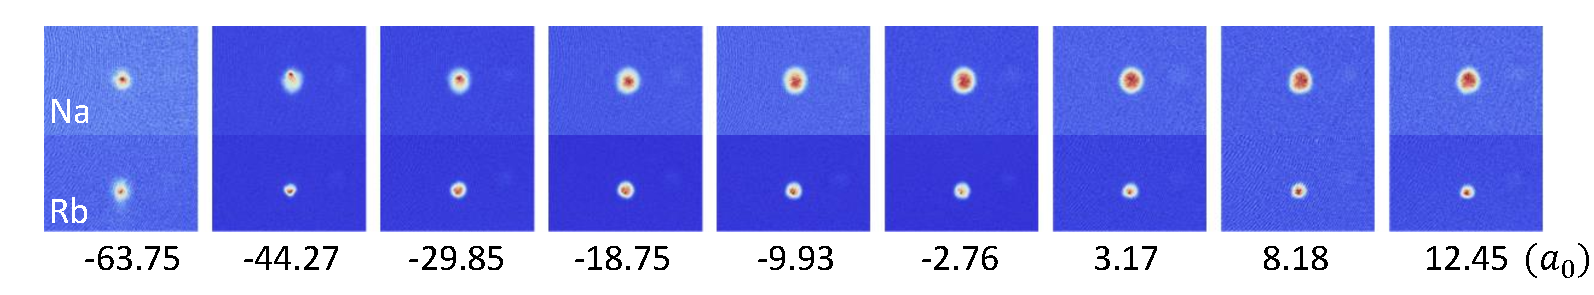
\includegraphics [width = 1 \linewidth]{dBEC_miscibility .pdf}
\end{center}
\caption[Na-Rb BEC mixture with various inter-species interaction]{With method introduced in Fig. \ref{ToF_dBEC_highBfield}, we scan the interspecies interaction to probe the miscibility of mixture BEC sample. The ToF duration in free space for Na(Rb) is 13(18) ms. From right to left, with $a_{\rm Na-Rb}$ gradually decreasing, the size of both Na and Rb shrinks. Moreover, a severe loss is detected for $a_{\rm Na-Rb}=-63.8 a_0$}
\label{dBEC_miscibility}
\end{figure}

% start droplet experiment (done: 2021年8月16日22:17:25)
Then, we notice Petrov's paper \cite{petrov2015}, in which he described a stabilization mechanism that could avoid the MF collapse by the so-called LHY correction. Meanwhile, we found Leticia's paper \cite{cabrera2018quantum} showing the experimental study of the ${}^{39}$K droplet. This work encourages us to re-do the experiment mentioned above again and try to find the droplet signal. So, that is the start point of our experiment. Our goal is to build the first hetero-nuclear droplet made of a mixture Na-Rb BEC.

% droplet in low field image (done: 2021年8月17日11:12:41)
At the very beginning, we only have absorption image in the low magnetic field, which considerably limit our ability to detect the droplet signal. Because quantum droplet's size is relatively small, typically less than 2-3 \(\mu m\). With this limited image method, we have to detect the signal after a long ToF. As we already know, the dynamics during the ToF would severely affect the sample's shape and size. We thus choose to do the ToF under 350 G magnetic field for 5 ms first, then switch down the magnetic field. After 8(13) ms ToF in the low magnetic field, we do a Na(Rb) absorption image. As shown in Fig. \ref{LowField_droplet}, we measure the sample's size and number. When the magnetic field is higher than 352 G, i.e. around \(a_{\rm Na-Rb}=0\), both Na and Rb show a constant size and number. When the magnetic field gradually decrease to 350.4 G, i.e. about -40 \(a_0\), the size of Na decreases; meanwhile, Rb size is almost unchanged. This phenomenon can be understood that Na has absorbed into Rb thanks to the miscible and attractive interaction. When the magnetic field decreases further, a severe loss shows up for both Na and Rb, mainly due to the three-body loss happening when the density gets high. Then when the magnetic field is across 350 G, sizes of both Na and Rb increase sharply upon the magnetic field. Here, we already find this abnormal expansion velocity of the sample. However, the explanation could be either three-body loss(heating) in a droplet sample or just BEC collapsing, which is hard to distinguish them.

% Low field image for droplet signal (done 2021年8月17日11:13:55)
\begin{figure}[htbp]
\begin{center}
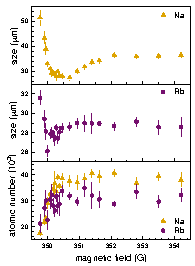
\includegraphics [width = 0.6 \linewidth]{LowField_droplet.pdf}
\end{center}
\caption[Try to detect droplet signal by low field image]{This figure shows our try at detecting droplet signals with a low-magnetic field absorption image. With the magnetic field decrease from 352 G to 350 G, we can see an apparent decrease in the size of both Na and Rb. This is thanks to the inter-species attractive interaction. Then, with a further decrease of the magnetic field, we see steep inflation of sample size and severe loss.}
\label{LowField_droplet}
\end{figure}

% problem with low field image (done 2021年8月17日11:34:04)
With this measurement, we cannot make conclusion that we catch the signal of droplet. Whatever, we spent only two weeks doing the fast test and making the decision, which is judicious from the current point of view. Besides the above mentioned reasons, we have to suspect the destructive dynamics of the sample during the ToF when the magnetic field switching down. Because the droplet sample have a density even 10 times larger than a typical BEC sample, we have to treat this ToF process very carefully. So, what we need is a new image method which can directly capture the sample under a high magnetic field (around 350 G). We stop our experiment and try to design a image method working under high magnetic field. First, we want to try the Faraday image. We do the calculation, trying to find the rotation angle for our sample. However the calculation shows that we need an EMCCD to get enough SNR, which is out of our afford. So we turn back to try the absorption image under a high magnetic field. There were two problems: we need to find a cycling (or almost-cycling) transition under 350 G; another is we need to handle the sample with extremely high optical density (OD), around 10 to 50 for the Rb sample. We calculate and conceive all possible image scheme, such as two examples shown in Fig. \ref{image_scheme_II}. We first try a $90\%$ almost-cycling transition (shown in (a) of Fig. \ref{image_scheme_II}), then we turn to the other one since even the $10\%$ leakage cause hard calibration of the sample's OD. For another problem, we use the partial transferring \cite{ramanathan2012partial}. We will detailly discuss then in the apparatus chapter (Chap. \ref{Chap_Apparatus}).

% non-cycling image scheme (done: 2021年8月16日11:03:34)
\begin{figure}[htb]
\begin{center}
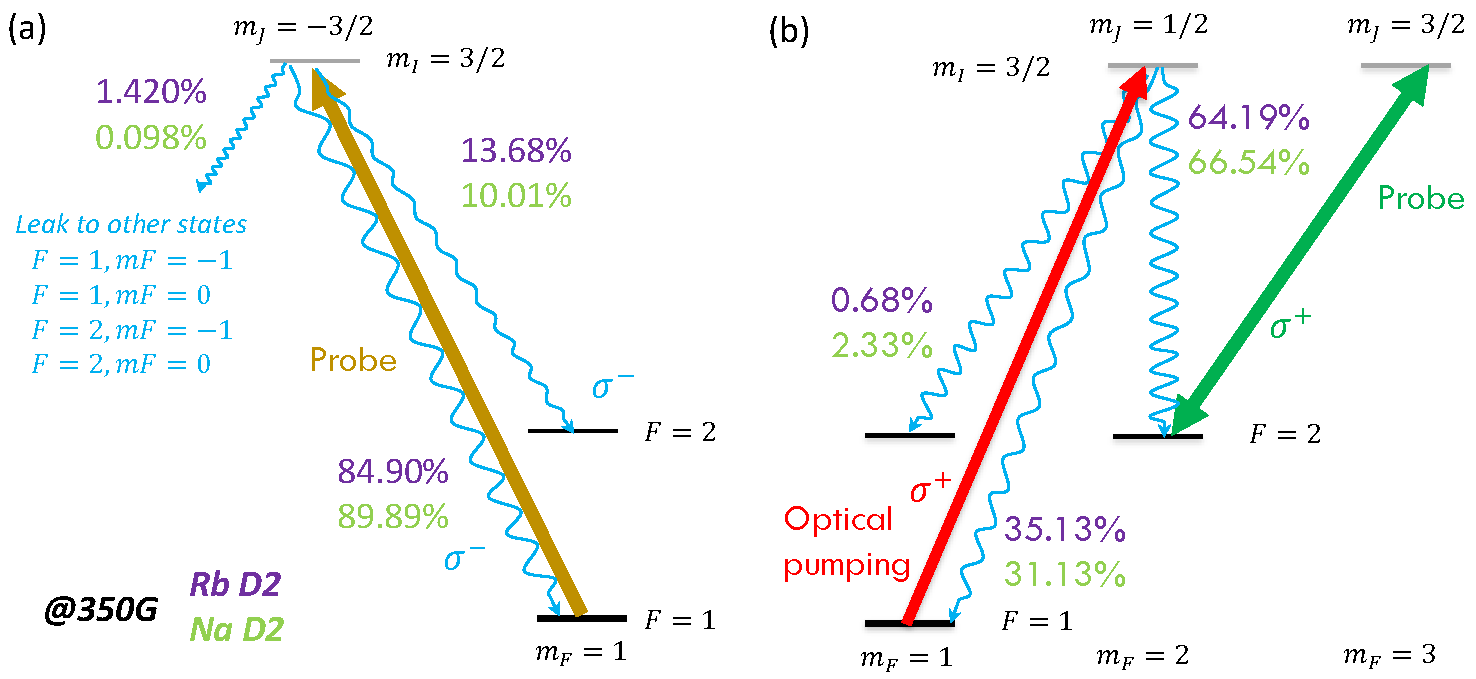
\includegraphics [width = 0.9 \linewidth]{image_scheme_II.pdf}
\end{center}
\caption[Two image schemes for Na(Rb) $\ket{F=1,m_F=1}$ state under 350 G]{(a) non-cycling image scheme for Na(Rb) $\ket{F=1,m_F=1}$ state. (b) After partially pumping the $\ket{F=1,m_F=1}$ atoms to the cycling transition for $\ket{F=2,m_F=2}$ state. The calculation is under 350 G magnetic field.}
\label{image_scheme_II}
\end{figure}

% non-cycling image method in high field (done 2021年8月17日12:03:41)
In July 2018, We first chose the non-cycling transition with \(90\%\) probability back to the original state. With this imaging method on Na, we get the first signal of a droplet. Even though we know it is not a droplet (since the magnetic field is 350.089G, which is higher than the mean-field collapse boundary 349.978 G). We are very close to the collapse bound. However, due to the limited ToF duration and image resolution, we thought that was the droplet. As shown in Fig. \ref{droplet_signal_Na_first}, this deep attractive double BEC already shows its tiny expansion property. Then, we are encouraged and build the Rb high-magnetic-field (HF) image with the beat locking method. We found it hard to use scheme (a) since the high OD cause the sensitivity of the OD we obtain upon the image duration. So we switch to image scheme (b). 

% non-cycling image for droplet signal (done 2021年8月17日12:04:16)
\begin{figure}[htb]
\begin{center}
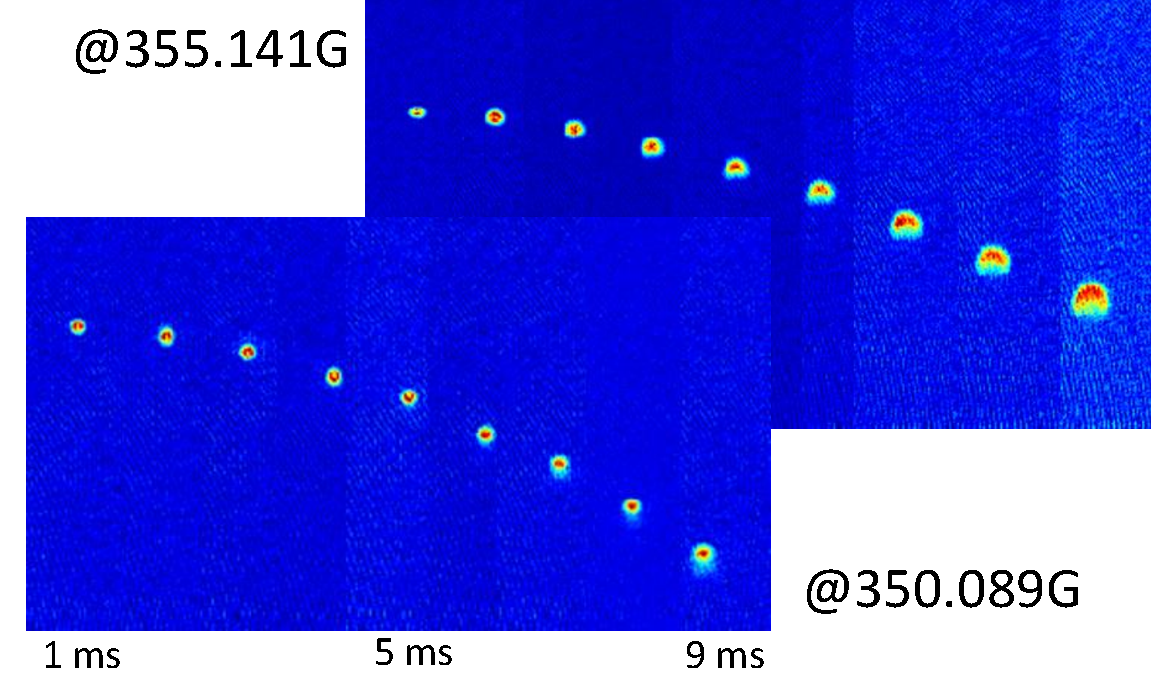
\includegraphics [width = 0.7 \linewidth]{droplet_signal_Na_first.pdf}
\end{center}
\caption[non-cycling absorption image for droplet signal]{Na absorption image with non-cycling scheme. Signal at 350 G show clear size shrinking and shape turning to sphere.}
\label{droplet_signal_Na_first}
\end{figure}

% found magnetic field gradient (done 2021年8月17日12:22:02)
Thanks to images for both species, we discover the magnetic gradient affecting the droplet sample. As shown in Fig. \ref{Apparatus_gradient-compen}, the gradient applies on Na and Rb generate different forces due to different mass and dipole. The mixture sample tends to be torn apart. So, for observing a better droplet signal without the effect of a gradient, we compensate the gradient with another single-coil (right panel of Fig. \ref{Apparatus_gradient-compen}). By measuring the accelerations of both Rb and Na, we can choose the best compensation point. After solving this problem, we obtain the non-expansion signal of the droplet clearly, as shown in Fig. \ref{first_signal_both}. We use an imbalanced number case; the Na number is much larger than Rb. A clear, bright spot shows up at the centre of the Na BEC, which shows the smoking-gun signal for the droplet.

% first signal for both case (done 2021年8月16日11:42:23)
\begin{figure}[htbp]
\begin{center}
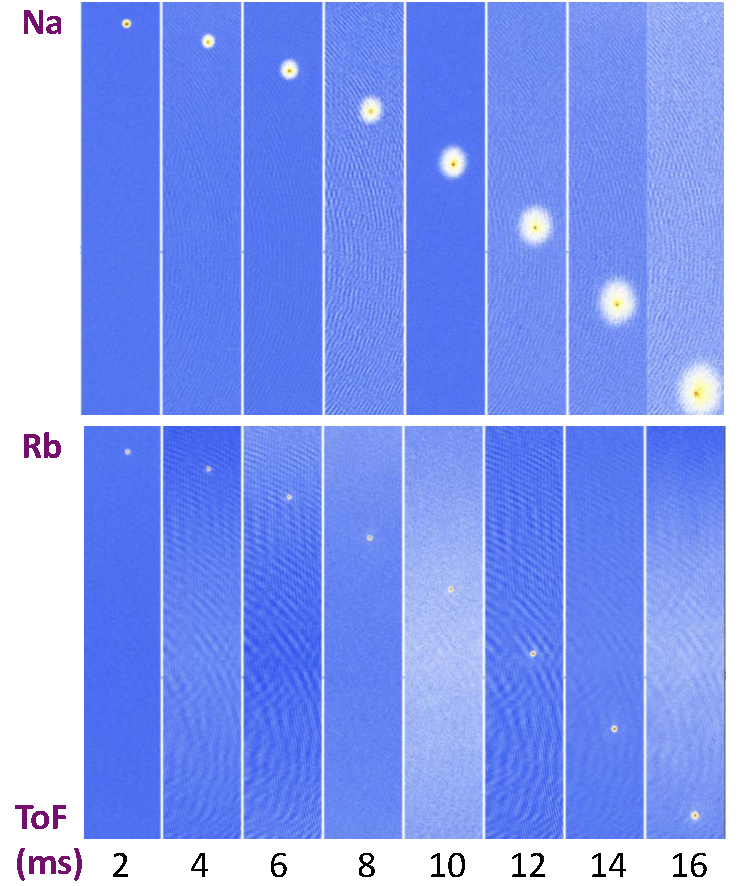
\includegraphics [width = 0.7 \linewidth]{first_signal_both.pdf}
\end{center}
\caption[Droplet signal of number imbalanced case]{Na and Rb droplet signal under 349.826 G. atomic number for Na(Rb) is $9\times10^4$ ($3\times10^4$). A clear, bright spot shows up inside the BEC surrounding of Na sample.}
\label{first_signal_both}
\end{figure}

% signal under 3x image system with Na Rb both partial pump method (done 2021年8月17日12:32:51)
After the detection we made in Fig. \ref{first_signal_both}, we find that the image resolution is limited since the original image system with 3x magnification has a resolution of 4 $\mu$m and pixel corresponding size 2.1 $\mu$m. Both parameters are comparable to the size of the droplet and even larger than it. So, we determined to upgrade our image system. We first choose the set-up of the microscope and the zoom lens system from Navitor. This system offers a magnification changing from 0.8 to 12 times, which is enough for our measurement. Meanwhile, we use a Mitutoyo long-working distance microscope to upgrade the image resolution. After all these upgrades, we achieve a 15x image system with a resolution of around 2 $\mu$m. Details can be found in Sect. \ref{image_system}.

% problem with FR (done 2021年8月17日12:42:35)
In June of 2019, after finishing all the technical problems, we started to take data for the droplet sample. We measured the non-expansion signal and studied the phase diagram. Besides the liquid droplet phase, we also study the gas phase, trying to understand the abnormal expansions. Details can be found in Chap. \ref{Chap_droplet}. Then, we meet the big problem that the experimental measurement of the phase diagram has a 300 mG discrepancy compared to the theoretical calculation. Even we do a more careful compensation of the magnetic field and number calibration, the discrepancy is still there. Finally, we doubt the accuracy of our Feshbach resonance parameter, so we re-do the FR calibration \cite{guo2021tunable}. This is an individual story as depicted in Chap. \ref{Chap_Feshbach}.

% some comments (done 2021年8月17日13:02:27)
I summarize the journey of studying quantum droplets as follows: first, the goal of this study is passive since we did not figure out what we want to study at the very beginning. A clear goal is vital to guide and push the following movement, such as technique upgrading or numerical simulation. Second, the review work done at the first phase is not broad enough. We only focus on the already existing experimental works and theories. Actually, finding the connection between other fields is essential and could guide the following working direction. Third, my attitude to the \textit{numbers} is not serious that caused using of the unverified parameters. This pulled our leg for a long time and finally causing the degrading of this work. In all, it is a good lesson to not only my research career but also to my daily life, from the attitude to details to the way of thinking and doing.

\section{Outlooks}
\label{sec:outlooks}

% Problem of research now
The biggest difficulty and problem of our experiment is that it is impossible to obtain a sample with a sufficient and stable lifespan. Because the experiment uses the ToF method, if the atomic group flies too far, both the gradient of the magnetic field and the resolution of the imaging will be further affected, thereby limiting the detection time. The improved scheme can refer to the Italian paper and adopt the method of light well levitation. It should be noted that the trap effect of levitation needs to be evaluated, so as to avoid the unwanted effect of additional traps. Another problem is the excessively high three-body loss rate. Because the density of the droplet is generally much higher than the gaseous BEC, about one to two orders of magnitude. Therefore, the three-body loss rate is higher by $10^2$ to $10^3$. For such a serious loss, it can only be achieved by preparing a droplet with a weaker bond to reduce the density of its equilibrium state. The negative effect of this is that the requirements for the number of atoms are correspondingly increased. Our new device uses 2D-MOT to increase the atomic number of Na, which may have the opportunity to prepare quantum droplets with more atomic numbers.

% low dimension as new direction
On the existing experimental devices, the experiments we may explore mainly include the study of low-dimensional quanutm droplets. Refer to petrov and other papers, for 2D or 1D systems, it is relatively easier to implement droplets, which stems from the fact that the quantum fluctuation of low-dimensional systems is more important than the MF part. For example, the formation conditions of 2D droplets will be more relaxed than 3D. $\delta g$ does not need to be less than 0, it can also form a droplet phase. In addition, 2D is more abundant, and there are many interesting research content waiting to be discovered.

% theory problems and possible solutions
From the theoretical point of view, Petrov's theory \cite{petrov2015} has a loophole, which was discussed by \cite{Hu2020, Hu2020a}. As we present in Chap. \ref{Chap:theory}, the integral of the low-momentum imaginary region of the excitation spectrum is ill. This may hide a more profound physics. The problem can be severe when we tune $\delta g$ to be even negative, finally deviating from the weak attractive MF condition. Then, we must quest the microscope formation mechanism of the quantum droplet. One theory proposes the Bose pairing mechanism, which imitates the BCS theory providing a new field of pair of Boson. For a low dimension system, the Bose-pairing can form naturally. However, for the 3D case, the bound state formation is subtle. How to design an experiment to verify these new theories is essential. For example, for the theory of Bose pairing, it may be possible to use brag spectroscopy to detect the excitation of the pair to verify.

% experiment outlooks #1
In addition, starting from the already formed droplet, we can also consider its improvement or inspiration for other experiments. For example, droplet leads to a very good overlap of Na Rb. Considering this, we try to use this as a starting point to improve the formation rate of Feshbach molecule. Our experiments show that this effect is not very obvious. In addition to the limitations of experimental methods, theoretically it may be related to a multi-body system such as sample itself is condensate. Then this system can be used as a good platform to detect the transition from few to many bodies.

% closing
In short, quantum droplet is a small branch that studies many-body physics. Its significance is to raise the status of LHY correction to a dominant position, not just a correction. Compared with the measurement of other previous experiments, this has a very extraordinary significance. Then, for such a new phase, dig out more characteristics, so that it can become a very meaningful platform for in-depth study of pure quantum effect such as LHY or above LHY. The unique cleanness and easy control of the cold atom experimental system will bring excellent solutions for the study of many-body physics and further quantum simulations.

\chapterend

